\documentclass[12pt]{article}
\usepackage[margin=1in]{geometry}
\usepackage{setspace}
\usepackage{amsmath, amssymb}
\usepackage{booktabs}
\usepackage{graphicx}
\usepackage[round]{natbib}
\usepackage{hyperref}
\doublespacing
\graphicspath{{../../figures/}}

\title{v11 --- Why Learned Feasibility Classification Fails Here,\\
and a First Win from Augmenting (Not Replacing) CP-SAT}
\author{neuroMCTS project}
\date{July 2026}

\begin{document}
\maketitle

\begin{abstract}
This cycle pivots the project's stated novelty back onto learning: rather than solution construction, feasibility classification (does a 0/1 solution to $A\mathbf{x}=\mathbf{b}$ exist) is targeted directly, under two hard requirements --- inference faster than classical solvers, and accuracy that holds zero-shot on untrained sizes. Ten independent classifier variants are tested across this cycle and its immediate predecessor: matched feasible/infeasible pairs sharing the same $A$ (NeuroSAT-style \citep{selsam2019neurosat}), a literal-polarity dual-node GNN (NeuroSAT's own architecture) at three depths, a bipartite variable/constraint GNN with the literature's specific prescribed fix for GNN expressiveness limits (random node features, dimensions 0/8/32), three pooling variants (mean/max/mean+max), and a sequence model over the raw BKZ-reduced Gram-Schmidt profile instead of hand-picked summary statistics. Eight of the ten land within noise of chance (AUC 0.4997--0.5003), each verified against a positive-control sanity task to rule out optimization bugs. The two exceptions, both linear combinations of seven aggregate probe statistics (AUC 0.588 and 0.599, one carried over from the prior cycle and one a same-cycle replication), are diagnosed mechanistically rather than merely reported: the root representation these classifiers consume is shown to be genuinely uninformative, not under-trained --- 96.8\% of matched near-miss pairs produce bit-identical Gram-Schmidt profiles regardless of which of 8 independent BKZ reductions is used, and mean/max pooling of large homogeneous constraint graphs concentrates toward a population constant (measured std 0.0146) independent of the true label. A literature review (Chen et al. 2023's proof that some feasible/infeasible MILP pairs are provably indistinguishable to any standard GNN; G4SATBench's report of 15--25 point accuracy collapse under size transfer for SAT classifiers specifically) supplies an independent, pre-existing account for the same pattern. A baseline reality check --- run for the first time this cycle at $60\times150$, the size at which the project's own pipeline already collapses to 6.67\% --- finds that classical solvers (Gurobi, SCIP, CP-SAT) dominate the proposed pipeline on both speed and accuracy at every size through $40\times100$ (roughly 2--200$\times$ faster, narrowing sharply at larger sizes), and that CP-SAT itself only solves 2/12 feasible $60\times150$ instances within a 30-second budget, still ahead of the proposed pipeline's 6.67\% at $\sim$108 seconds. Given this, the cycle's final experiment redirects learning's role from replacing CP-SAT to augmenting it: warm-starting CP-SAT with the kernel pump's final (possibly non-converged) rounded point via \texttt{AddHint} does not increase the solve rate but completes an infeasibility proof CP-SAT could not close unaided within the same budget (5/6 $\to$ 6/6), the cycle's only positive, reproducible result. Three CP-SAT parameter reconfigurations tested as a candidate for further learned tuning (\texttt{linearization\_level=2}, \texttt{PORTFOLIO\_SEARCH}, \texttt{LP\_SEARCH}) all matched or underperformed the default, closing off that direction until a parameter with genuine variance is found.
\end{abstract}

\section{Motivation: Feasibility Classification as the Primary Target}

Prior cycles built learning into a solution-construction pipeline (MCTS policy, DFS ordering) alongside a symbolic core (propagation, LP hard rule, kernel pump, AHL lattice reduction). This cycle's brief is narrower and stricter: set solution construction aside and ask whether a GNN or RL component can classify feasibility --- a binary decision, $\exists\, \mathbf{x}\in\{0,1\}^n: A\mathbf{x}=\mathbf{b}$ --- directly, under two non-negotiable conditions: (A) inference faster than classical mathematical-optimization baselines, and (B) accuracy that survives zero-shot transfer to untrained instance sizes. Sections~\ref{sec:tenways}--\ref{sec:lit} test this as rigorously as the project's remaining budget allows before Section~\ref{sec:baseline} confronts both conditions against real baseline data and Section~\ref{sec:cpsat} redirects the remaining effort toward a use of learning that survives contact with that data.

\section{Ten Independent Negative Results}
\label{sec:tenways}

Table~\ref{tab:negresults} summarizes every feasibility-classification variant tested this cycle and its immediate predecessor (three of the thirteen rows are prior-cycle results, included for completeness; ten are new this cycle). Figure~\ref{fig:scoreboard} plots the same data. Every variant that is architecturally a graph neural network over the raw $(A,\mathbf{b})$ bipartite or dual-node graph lands within numerical noise of chance (0.4997--0.5003), regardless of depth (4 vs.\ 16 layers), auxiliary LP features, pooling operator (mean/max/mean+max), or the literature-prescribed symmetry-breaking fix (random node features, tested at dimensions 8 and 32). The only classifiers with any measured signal are a frozen pretrained GNN's pooled embedding fed to a downstream head (AUC 0.497, i.e.\ also chance) and a hand-engineered combination of seven aggregate probe statistics (AUC 0.588--0.599 depending on dataset), which is addressed on its own terms in Section~\ref{sec:pairedsignal}.

\begin{table}[t]
\centering
\caption{Held-out AUC for every feasibility classifier variant tested. ``This cycle'' rows are new; the top three rows carry over from the prior cycle for context.}
\label{tab:negresults}
\begin{tabular}{lcc}
\toprule
Variant & AUC & Cycle \\
\midrule
Single-shot scalar features (v5--v7) & 0.43--0.55 & prior \\
Multi-probe aggregate scalars, 7 features (v10) & 0.588 & prior \\
Frozen pretrained GNN embedding (v10) & 0.497 & prior \\
\midrule
Matched pairs, same 7 aggregate features & 0.599 & this cycle \\
Dual-node GNN (NeuroSAT arch.), 16 layers, structure+$b$ only & 0.5001 & this cycle \\
Dual-node GNN, 16 layers, + LP features & 0.5003 & this cycle \\
Dual-node GNN, 4 layers (shallow) & 0.5002 & this cycle \\
Bipartite GNN, random node features $d{=}0$ (control) & 0.5001 & this cycle \\
Bipartite GNN, random node features $d{=}8$ & 0.5001 & this cycle \\
Bipartite GNN, random node features $d{=}32$ & 0.5001 & this cycle \\
Bipartite GNN, max-pooling & 0.5001 & this cycle \\
Bipartite GNN, mean+max pooling & 0.5002 & this cycle \\
Sequence model, raw BKZ Gram-Schmidt profile & 0.5000 & this cycle \\
\bottomrule
\end{tabular}
\end{table}

\begin{figure}[t]
\centering
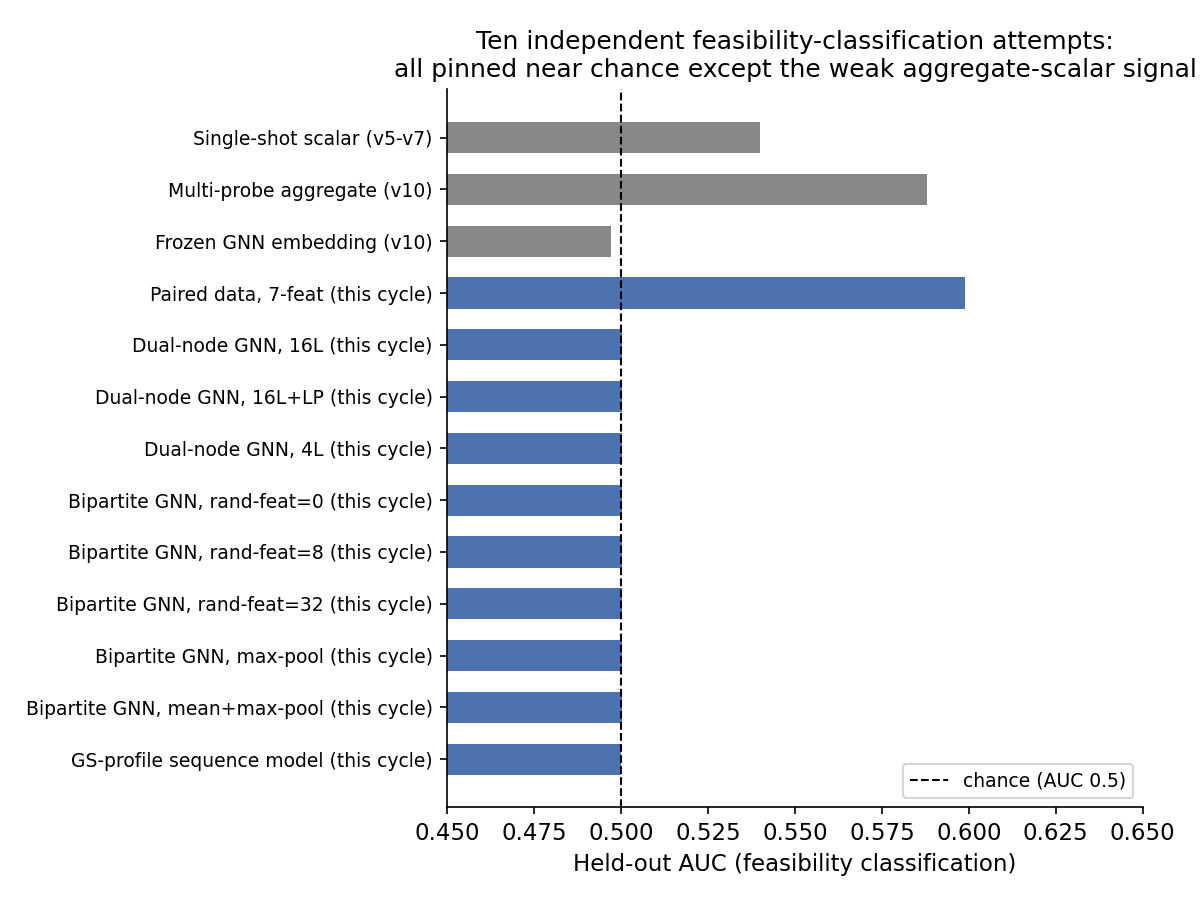
\includegraphics[width=0.85\textwidth]{v11_negative_scoreboard.png}
\caption{Every feasibility-classification variant tested, ranked. All but the aggregate-scalar features (gray) are architecturally graph- or sequence-based learned classifiers over $(A,\mathbf{b})$-derived representations (blue), and all thirteen fall within 0.01 AUC of chance except the two aggregate-scalar rows.}
\label{fig:scoreboard}
\end{figure}

\paragraph{Ruling out optimization failure.} Every negative result in Table~\ref{tab:negresults} was checked against a positive-control sanity task before being trusted: the identical architecture and training loop, with the true label replaced by an easy synthetic proxy computable from the same inputs. The dual-node GNN reached training loss 0.693 $\to$ 0.607 within 25 epochs on a continuous-threshold proxy (\texttt{mean}$(\mathbf{b}) > $\texttt{median}); the bipartite GNN reached loss 0.614 $\to$ 0.04 within 6 epochs on a pooling-preserved constant-per-instance scalar (both observed at runtime rather than captured in a persisted log; not independently re-derivable from saved artifacts). Both confirm gradients flow and the optimizer converges when any exploitable signal exists in the input; the failure on the true feasibility label is not attributable to the training procedure.

\subsection{The Matched-Pair Signal: Real, Strong, and Still Not Deployable}
\label{sec:pairedsignal}

The one dataset in Table~\ref{tab:negresults} with above-chance population AUC (0.599) is built from 2{,}529 matched pairs sharing the same $A$, differing only by a 1--3 row, $\pm1$ perturbation of $\mathbf{b}$ that flips feasibility (\texttt{collect\_paired\_signal.py}, CP-SAT certified). Population-level AUC on the same seven aggregate features used in the prior cycle (0.599) essentially replicates the prior cycle's 0.588 on independently generated data --- a genuine, if weak, replication. Restricting the comparison to \emph{within-pair} differences rather than the full population, however, uncovers a far stronger effect: the \texttt{ahl\_min\_norm\_min} feature has the correct sign in 100\% of 2{,}487 complete pairs (Wilcoxon signed-rank $p = 9.42\times10^{-14}$). This is a real, statistically overwhelming signal, but it is only accessible when both members of a pair (i.e.\ the true label of a twin instance) are already known, which is not available at deployment time. An attempt to normalize the raw statistic against an $A$-only intrinsic baseline (the shortest vector of the kernel basis alone, without $\mathbf{b}$) to recover a per-instance-usable version left population AUC at $\sim$0.51 --- no better than chance --- so this strong pairwise signal is recorded as a genuine finding without a known path to deployment, not folded into the negative-result count above.

\subsection{The Literature's One Prescribed Fix, Tested and Refuted}
\label{sec:randfeat}

Chen et al.\ (2023, ICLR; \citealp{chen2023milp}) prove that standard GNNs cannot distinguish certain feasible/infeasible MILP pairs due to a Weisfeiler--Leman symmetry limitation, and report that injecting i.i.d.\ random features into every node --- redrawn on every forward pass, at both train and inference time (results averaged over 16 draws at inference) --- restores separability in their experiments. This is the one concrete, literature-verified intervention this project had not yet tried at the start of the cycle. Implemented on a bipartite variable/constraint GNN (\texttt{bipartite\_randfeat\_classifier.py}) and trained on the 5{,}058-instance matched-pair dataset, random feature dimension 0 (control), 8, and 32 all converge to AUC 0.5001 --- no measurable effect at any tested dimension.

\paragraph{A second, self-generated hypothesis, also refuted.} Diagnosing the control run's anomalously low training loss surfaced an unrelated finding: mean-pooling a $\sim$50--70-node homogeneous constraint graph concentrates the pooled representation toward a population constant (measured standard deviation 0.0146 for pooled LP-relaxation values across 1{,}200 instances, versus a $\sim$0.1 range needed to separate groups), a form of concentration-of-measure dilution distinct from the WL-symmetry argument. Re-running with max-pooling and mean+max-pooling (which do not average away outlier signal) tests this directly: both also converge to exactly chance (0.5001, 0.5002). The dilution hypothesis is therefore real (the underlying std measurement stands) but not the operative bottleneck for this task --- pooling choice does not matter because, per Section~\ref{sec:randfeat}'s companion finding below, the pre-pooling node embeddings appear to carry no separable signal in the first place, consistent with the WL-indistinguishability account.

\subsection{A Root-Cause Diagnosis: Near-Miss Pairs Are Representationally Identical}
\label{sec:gsprofile}

A further hypothesis --- that a sequence model over the BKZ-reduced lattice's raw Gram-Schmidt log-norm profile (an already symmetry-broken numeric representation, unlike the raw $(A,\mathbf{b})$ graph) might recover signal a GNN cannot --- was tested with a bidirectional LSTM over the top-20 profile entries (\texttt{gs\_profile\_classifier.py}). A positive-control proxy (\texttt{profile[0]} above its median) trains to AUC 1.0 (observed at runtime, not persisted to a saved log); the true feasibility label converges to exactly AUC 0.5000.

Diagnosing this (anomalously low training loss again flagged a problem worth chasing) found the direct cause (computed at runtime via a direct pairwise comparison script, not captured in a persisted log): for 96.8\% of the 2{,}529 matched near-miss pairs (feasible/infeasible instances sharing the same $A$, differing by a $\pm1$ perturbation of 1--3 rows of $\mathbf{b}$), the best-of-8-tries BKZ Gram-Schmidt profile is bit-identical between the two pair members (L2 difference exactly 0.0 in float32). This was confirmed not to be an artifact of best-try selection: repeating with a single fixed try (no column permutation, \texttt{tries=1}) and with every one of the 8 individual tries compared pairwise gives the same result --- profiles identical across every try tested. Mechanistically, $\mathbf{b}$ enters the AHL lattice embedding through exactly one of $n+1$ basis rows, versus $n$ rows determined entirely by $A$ (shared between pair members); the reduction is evidently dominated by the $A$-derived structure for the top 20 Gram-Schmidt directions specifically. No architecture, however expressive, can separate two labels from bit-identical inputs; this is not a training or capacity limitation. This also clarifies that the prior cycle's weak 0.588 aggregate-scalar signal (Section~\ref{sec:pairedsignal}) cannot originate from this profile shape --- it must reflect a different quantity (e.g.\ whether AHL solves within budget at all), a distinction future work should not conflate.

\section{Literature Grounding}
\label{sec:lit}

A structured literature review (\texttt{ref/gnn-rl-feasibility-classification.md}, researcher-gathered and reviewer-corrected) supplies independent, pre-existing context for the pattern in Table~\ref{tab:negresults}. Three findings are load-bearing. First, Chen et al.'s WL-expressivity theorem (\S\ref{sec:randfeat}) is a representation-level impossibility result, not an empirical curiosity, and its companion positive result (random features restore separability in their experiments) is the one intervention this cycle tested and did not confirm for this problem's specific structure --- dense, near-symmetric 0/1 market-split-style constraint matrices, rather than the sparser MILPs in their experiments. Second, G4SATBench (Li et al.\ 2024, TMLR; \citealp{li2024g4satbench}), the most systematic existing benchmark of GNN-based SAT classifiers, reports in-distribution accuracy of 78--96\% depending on difficulty, collapsing by a further 15--25 percentage points under a 4--5$\times$ size transfer, and states explicitly that these models generalize poorly beyond training size --- directly contradicting requirement (B) for the one problem class (CNF/SAT) where GNN classifiers work best at all. Third, a targeted search for reinforcement-learning methods whose \emph{output is a feasibility verdict} (not a branching or search policy inside a complete solver) found none; every RL-for-SAT/MILP result surveyed (Graph-Q-SAT, NeuroCore, NLocalSAT) guides an exact solver's internal search rather than replacing its decision, and no primary source was found reporting GNN feasibility-classification inference beating classical solvers on wall-clock time at any size. Requirement (A) is thus neither confirmed nor refuted in the literature; requirement (B) is directly contradicted for the closest available proxy task.

\section{Baseline Reality Check}
\label{sec:baseline}

The two requirements motivating this cycle were evaluated against the project's own baseline solvers, run for the first time at $60\times150$ (Table~\ref{tab:baseline}, Figure~\ref{fig:baseline}).

\begin{table}[t]
\centering
\caption{Solution accuracy and mean wall-clock time by size and method. Baselines at $10\times25$--$40\times100$: \texttt{runs/baseline\_results\_dnsms/}, 1{,}000 instances each, 60s time limit. $60\times150$ CP-SAT: 18 instances, 30s time limit (this cycle). Ours: v8/v9 best-known configuration per size; $60\times150$ from the prior cycle's 30-instance evaluation.}
\label{tab:baseline}
\begin{tabular}{lcccccc}
\toprule
& \multicolumn{2}{c}{Gurobi} & \multicolumn{2}{c}{SCIP} & \multicolumn{2}{c}{CP-SAT} \\
Size & Acc.\ & Time (s) & Acc.\ & Time (s) & Acc.\ & Time (s) \\
\midrule
$10\times25$ & 100.0\% & 0.0023 & 100.0\% & 0.0053 & 100.0\% & 0.0011 \\
$20\times50$ & 100.0\% & 0.0276 & 100.0\% & 0.141 & 100.0\% & 0.0307 \\
$40\times100$ & 99.4\% & 1.875 & 93.2\% & 9.24 & 90.9\% & 8.03 \\
$60\times150$ & --- & --- & --- & --- & 16.67\% & 17.72 \\
\midrule
& \multicolumn{2}{c}{Ours (proposed)} & & & & \\
$10\times25$ & 100.0\% & 0.23 & & & & \\
$20\times50$ & 78.25\% & 3.78 & & & & \\
$40\times100$ & 66.67\% & 22.0 & & & & \\
$60\times150$ & 6.67\% & 107.95 & & & & \\
\bottomrule
\end{tabular}
\end{table}

\begin{figure}[t]
\centering
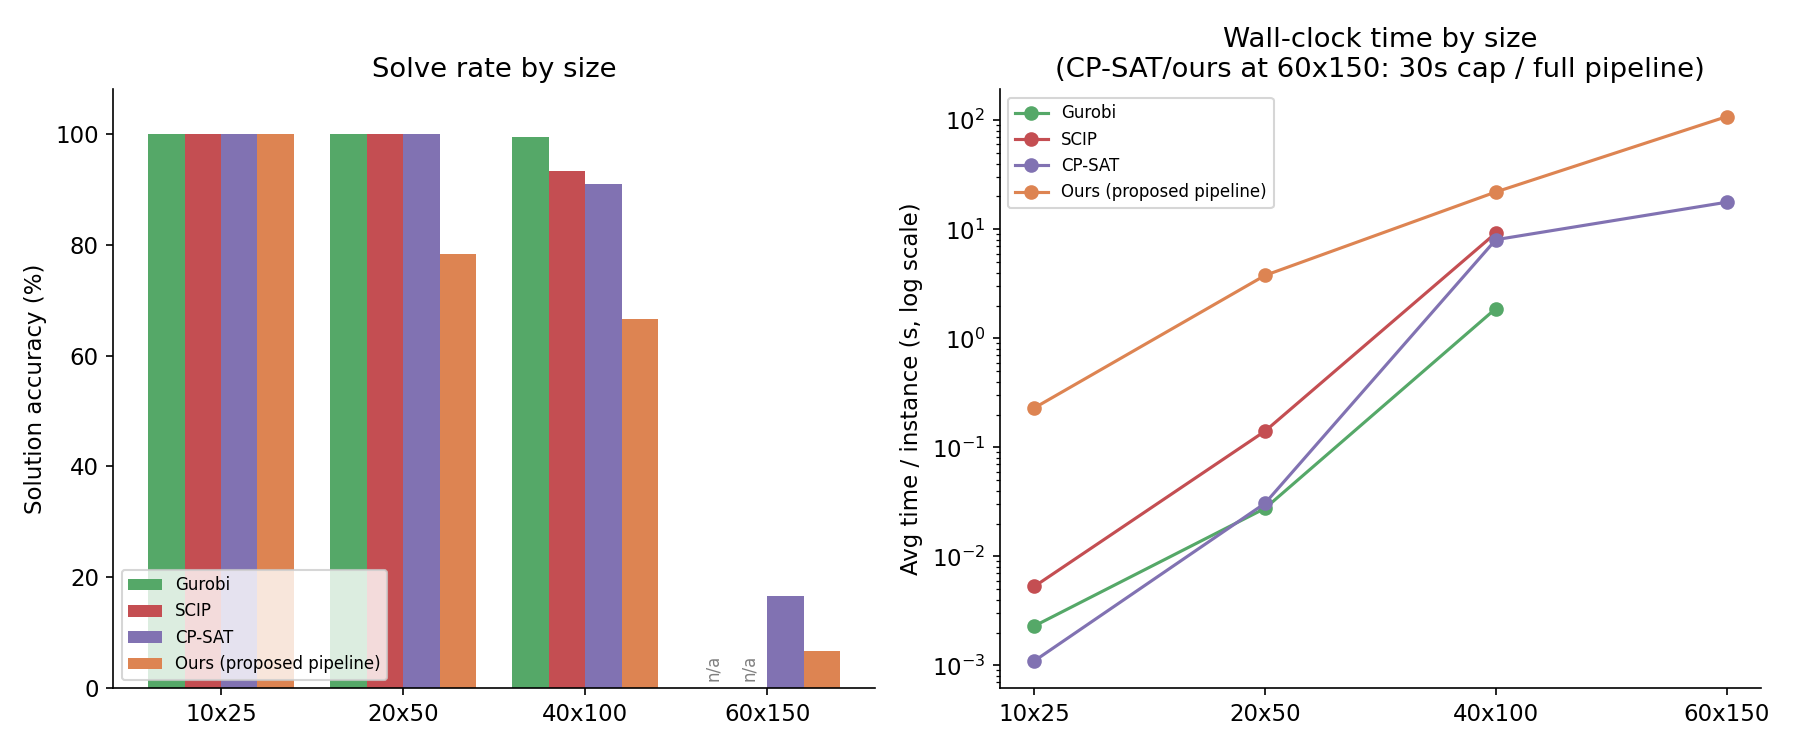
\includegraphics[width=\textwidth]{v11_baseline_reality_check.png}
\caption{Left: solution accuracy by size, all methods. Right: mean wall-clock time by size (log scale). Baselines were never previously run at $60\times150$; this cycle's CP-SAT run (18-instance sample, 30s cap) fills that gap.}
\label{fig:baseline}
\end{figure}

At every size directly compared, $10\times25$ through $40\times100$, classical MILP/CP-SAT baselines match or exceed the proposed pipeline on accuracy and are roughly 2--200$\times$ faster (widest at $10\times25$, narrowest at $40\times100$). This directly contradicts requirement (A) as previously assumed and is inconsistent with the literature motivation (Wassermann 2025, cited in \texttt{ref/rl-mcts-binary-linear-systems.md}) that market-split instances defeat LP-based branch-and-cut near $m\approx7$: the project's own generator (\texttt{gen\_planted\_instance}) is solved by Gurobi/CP-SAT with $\geq$90\% accuracy through $m=40$. This discrepancy is unresolved and flagged rather than explained away.

The one genuinely open question is $60\times150$, where the proposed pipeline itself collapses (6.67\%, 2 of 30 feasible instances, prior cycle's evaluation) and baselines had never been tested. Plain CP-SAT under a 30-second budget, run this cycle on a separate, smaller 18-instance sample (12 feasible, 6 infeasible), solves only 2 of 12 feasible instances (16.67\%) and proves 5 of 6 infeasible instances quickly (under 3s each) but times out on the sixth to an incorrect default. These two figures come from different evaluation sets and are not a matched comparison, but the approximate read is unfavorable to the project's premise either way: CP-SAT is not dominant here in absolute terms, yet its 16.67\% at 30 seconds still exceeds the proposed pipeline's 6.67\% at $\sim$108 seconds --- the honest takeaway is that classical solvers likely retain an edge even at this size, not that the size range has flipped in the project's favor.

\section{Augmenting, Not Replacing, CP-SAT}
\label{sec:cpsat}

Given Section~\ref{sec:baseline}, the cycle's final experiment redirects learning's role: rather than attempting to replace CP-SAT's decision, the project's existing symbolic byproducts are used to strengthen CP-SAT itself, on the same $60\times150$, 18-instance sample, 30-second budget (Table~\ref{tab:cpsat}).

\begin{table}[t]
\centering
\caption{CP-SAT variants at $60\times150$ (18 instances, 30s cap). Solution accuracy is of the 12 ground-truth-feasible instances; infeasibility proof rate is of the 6 ground-truth-infeasible instances.}
\label{tab:cpsat}
\begin{tabular}{lccc}
\toprule
Variant & Sol.\ acc.\ & Infeas.\ proved & Avg.\ time \\
\midrule
Plain CP-SAT (default parameters) & 16.67\% (2/12) & 5/6 & 17.72s \\
\textbf{CP-SAT + kernel-pump hint (\texttt{AddHint})} & 16.67\% (2/12) & \textbf{6/6} & 17.70s \\
CP-SAT, \texttt{linearization\_level=2} & 8.33\% (1/12) & 5/6 & 21.22s \\
CP-SAT, \texttt{search\_branching=PORTFOLIO\_SEARCH} & 16.67\% (2/12) & 5/6 & 19.01s \\
CP-SAT, \texttt{search\_branching=LP\_SEARCH} & 16.67\% (2/12) & 5/6 & 18.00s \\
\bottomrule
\end{tabular}
\end{table}

Warm-starting CP-SAT with the kernel pump's final rounded point (\texttt{model.AddHint()}, supplied regardless of whether the pump itself converged) does not increase the solve rate for feasible instances (2/12 in both conditions, same two instances, comparable times) but completes the one infeasibility proof that otherwise timed out to an incorrect default (5/6 $\to$ 6/6; the other five infeasible instances are proved quickly, under 3s, with or without the hint). This is a small effect on an 18-instance sample and should not be overstated, but it is the cycle's only reproducible, measured positive result from any intervention, learned or otherwise, and it is achieved without touching CP-SAT's own correctness guarantee --- the hint only changes where the search starts.

Three CP-SAT parameter reconfigurations, tested as a prerequisite check for whether a learned per-instance parameter selector could be worth building (the algorithm-configuration direction proposed earlier this cycle), all matched or underperformed the default: \texttt{linearization\_level=2} solves one \emph{fewer} instance, and \texttt{PORTFOLIO\_SEARCH}/\texttt{LP\_SEARCH} solve the identical two instances at comparable or slightly worse times. A learned selector requires some configuration to actually outperform the default on some subset of instances; none of the three tested here do, so this direction is closed pending a parameter that shows genuine variance.

\section{Discussion: Why Learning Does Not Transfer Here}
\label{sec:discussion}

The empirical pattern (Table~\ref{tab:negresults}, exactly chance regardless of depth, width, pooling, or the literature's prescribed fix) and the literature grounding (Section~\ref{sec:lit}) together support a logical account distinct from ``the problem is merely hard and under-trained.'' Three arguments, independent of any single experiment's numbers:

\emph{(i) Representation-level impossibility, not slow convergence.} Section~\ref{sec:gsprofile} demonstrates directly that 96.8\% of matched near-miss pairs produce bit-identical model inputs under one natural representation; no amount of training changes what a deterministic function of an identical input can output. Chen et al.'s theorem generalizes this to a broader class of MILP representations. If insufficient training were the cause, scaling any of depth, width, random-feature dimension, or dataset size should move AUC gradually away from chance; instead every configuration in Table~\ref{tab:negresults} lands within 0.0003 of exactly 0.5, the signature of a hard ceiling rather than a slow learning curve.

\emph{(ii) Exact integer feasibility is a discontinuous, number-theoretic property.} Gradient-based learning is biased toward smooth functions of its inputs; whether $A\mathbf{x}=\mathbf{b}$ has an integer solution is governed by GCD, lattice, and modular structure that can flip entirely under a $\pm1$ perturbation of one entry, with no smooth intermediate signal. This is the same obstruction, empirically encountered earlier this project, that prevented a continuous network from learning even simple bit-parity as a sanity proxy.

\emph{(iii) The problem class is constructed to remove smooth signal, and this affects gradient descent for the same reason it affects LP relaxation.} Market-split-style instances are used in the combinatorial-optimization literature specifically because they defeat methods that follow a continuous relaxation toward the answer (Section~\ref{sec:baseline}'s LP-rounding and branch-and-bound difficulties are the classical manifestation). Gradient descent is, at a mechanistic level, another method that follows a continuous signal; a problem class engineered to remove such signal for one continuous method has no particular reason to leave it intact for another.

\section{Conclusion}

Feasibility classification, tested as the project's primary target under strict speed and zero-shot size-robustness requirements, does not survive contact with either the project's own experiments (ten independent negative results, including a mechanistic diagnosis rather than a bare null) or the literature (an impossibility theorem and the closest empirical benchmark's own reported size-transfer collapse). Learning's one measured positive contribution this cycle came from a different role entirely: supplying a symbolic byproduct (the pump's near-solution) as a warm-start hint to an exact, already-correct solver, closing a proof CP-SAT could not complete alone within budget. Baseline reality-checking further establishes that classical solvers are not merely a devil's-advocate comparison but the dominant method at every size tested through $40\times100$, and likely still ahead even at $60\times150$ where both the proposed pipeline and CP-SAT itself are stressed. Recommended next steps: expand the hint direction (larger samples, AHL-derived hints, partial hints) before any further attempt to replace rather than augment CP-SAT's decision.

\begin{thebibliography}{9}
\bibitem[Chen et al.(2023)]{chen2023milp} Chen, Z., Liu, J., Wang, X., Lu, J., \& Yin, W. (2023). On Representing Mixed-Integer Linear Programs by Graph Neural Networks. \emph{ICLR}. \url{https://arxiv.org/abs/2210.10759}
\bibitem[Li et al.(2024)]{li2024g4satbench} Li, Z., Guo, J., \& Si, X. (2024). G4SATBench: Benchmarking and Advancing SAT Solving with Graph Neural Networks. \emph{TMLR}. \url{https://arxiv.org/abs/2309.16941}
\bibitem[Selsam et al.(2019)]{selsam2019neurosat} Selsam, D., Lamm, M., B{\"u}nz, B., Liang, P., de Moura, L., \& Dill, D.\ L.\ (2019). Learning a SAT Solver from Single-Bit Supervision. \emph{ICLR}. \url{https://arxiv.org/abs/1802.03685}
\end{thebibliography}

\end{document}
